\documentclass{../util/zariski}
\usepackage{tikz}
\usepackage{graphicx}
\usepackage{caption}
\usepackage{mathrsfs}
\usepackage{tikz-cd}
\usepackage{tikz}
\usetikzlibrary{shapes,patterns,positioning}
\usepackage{pgfplots}

\begin{document}
In this note we show that the topologists sine curve $\mathcal S$ can be defined in the setting of 
synthetic Stone duality (SSD) as introduced in \cite{synthetic-stone-duality}. 
We show that $\mathcal S$ is not path-connected. 
We will also show that $\mathcal S$ is $\mathbb I$-contractible. 
Note that any path-connected space is $\mathbb I$-contractible 
(Lemma 5.24 of \cite{synthetic-stone-duality}) but the converse thus does not hold. 
%\tableofcontents
\section{Preliminaries}
In \cite{synthetic-stone-duality}, synthetic Stone duality (SSD) was introduced. SSD consists of an extension of homotopy type theory by four axioms. In this section, we will recall the results from SSD that will be needed for later arguments. 

\subsection{The setting of SSD}
Note that all of the results we will present assume the axioms of SSD as in \cite{synthetic-stone-duality}. We will mention two of these axioms as they are useful for the purposes of this note. 
\begin{definition}
  Recall that a type is called \textbf{Stone} if it is 
  %the spectrum of a countably presented Boolean algebra. 
  a sequential limit of finite sets. The type of Stone types is denoted $\Stone$. 
  A type is called \textbf{compact Hausdorff} if it is the quotient of a Stone type by a Stone equivalence relation. The type of compact Hausdorff types is denoted $\CHaus$. 
\end{definition}
  
\begin{axiom}[Local choice]\label{AxLocalChoice}
  Given $X:\CHaus$ with $E,F$ arbitrary types, a map $f:X \to F$ and a 
  surjection $e:E \twoheadrightarrow F$, 
  there exists a Stone space $T$, a surjective map 
  $T\twoheadrightarrow X$ and an arrow $T\to E$ making the following diagram commute:
    \[\begin{tikzcd}
      T \arrow[d,dashed, two heads ] \arrow[r,dashed]&  E \arrow[d,""',two heads, "e"]\\
      X  \arrow[r, swap,"f"] & F
    \end{tikzcd}\]  
\end{axiom}

\begin{axiom}[Dependent choice]\label{axDependentChoice}
For all types $(E_n)_{n:\N}$ with surjections $E_{n+1}\twoheadrightarrow E_n$ for all $n:\N$, the projection from the sequential limit $\lim_kE_k$ to $E_0$ is surjective.
\end{axiom}
%From now on, we will assume these axioms. 

\subsection{The topology of compact Hausdorff spaces}
By \parencite[Cor 3.9]{synthetic-stone-duality}, we can define the type of closed propositions as follows:
\begin{definition}\label{dfnClosedOpen}
  A proposition $P$ is called \textbf{closed} if it is Stone. 
  The type of closed propositions is called $\Closed$.
  For $X$ a type and $A:X \to \Prop$ a subset, we call $A$ closed if $A$ factors over $\Closed$.
\end{definition}
%In \parencite[Rmk 1.20, Lemma 1.21]{synthetic-stone-duality} the following is shown:
\begin{remark}\label{ClosureClosedOpen}
  $\Closed$ is closed under countable conjunctions and finite disjunctions. Closed propositions are double-negation stable. 
  \parencite[Rmk 1.20, Lemma 1.21]{synthetic-stone-duality}
\end{remark}

From \parencite[Cor 4.9]{synthetic-stone-duality}, we recall the following:
\begin{lemma}\label{ExistsClosedSubsetDoubleNegation}
  Let $X:\CHaus$ and $A\subseteq X$ closed. Then $\exists_{x:X}A(x)$ is closed and equivalent to $A\neq \emptyset$. 
\end{lemma}

\begin{lemma}\label{CHausClosedImage}
  Let $X:\CHaus$ and $A\subseteq X$ a subset. Then $A$ is closed if and only if it is the image of a compact Hausdorff space. 
\end{lemma}
\begin{proof}
  Assume $A\subseteq X$ closed, by \parencite[Lemma 4.2]{synthetic-stone-duality}, $A$ is the image of some closed subset of a Stone space, which is itself Stone by \parencite[Cor 3.12]{synthetic-stone-duality}. If $f:X \to Y$ is a map of compact Hausdorff types, then $f(X) = \{ y : Y | \exists_{x:X} f(x) = y\}$, which is closed by \Cref{ExistsClosedSubsetDoubleNegation}.
\end{proof}
The compact Hausdorff spaces are indeed compact in the following sense:
\begin{lemma}\label{compactnessCHaus}
  Let $X:\CHaus$ and $C:\N \to X \to \Closed$. Then $\bigcap_{n:\N} C_n$ is inhabited as soon as for all $k:\N$ the finite intersection $\bigcap_{n<k} C_n$ is inhabited. 
\end{lemma}
\begin{proof}
  By \Cref{ExistsClosedSubsetDoubleNegation}, it is sufficient to show that the infinite intersection is nonempty as soon as the finite intersections are, which is \parencite[Lemma 4.5]{synthetic-stone-duality}.
\end{proof}

\subsection{The unit interval}
\begin{example}
  In \parencite[Thm 4.22]{synthetic-stone-duality}, it is shown that the interval $[0,1]$ of Cauchy reals as in \cite{Bishop} is compact Hausdorff. By rescaling, so is any closed interval $[a,b]\subseteq \R$ for any $a,b:\R$. Furthermore, in \parencite[Lemma 4.11]{synthetic-stone-duality}, it is shown that $\CHaus$ is closed under $\Sigma$, and hence in particular finite products. 
\end{example}
\begin{remark}\label{CauchyDfns}
  We recall that for the Cauchy reals, we can define the relations $<,\leq : \R \to \R \to \Prop$, and the standard functions 
 $\frac{1}{\cdot}:\R_{\neq 0} \to \R$ and
%  $|\cdot|,\sin,-:\R \to \R$ and 
  $\sin:\R \to \R$ 
%  $+,\cdot,\max,\min: \R \to \R \to \R$ 
%  Dfn 2.4 (+,times,max,-, 
%  Prop 2.13, 1/
% p 20 min, 
% p58 sin,cos
  % 2.7 defines nonnegative and positive and 2.10 defines >,\geq using these
  \parencite[Dfn 2.7,Dfn 2.10, Prop 2.13, p58]{Bishop}.
\end{remark}

  In \parencite[Cor 1.16]{synthetic-stone-duality}, Markov's principle is shown, which is equivalent to the following statement:
\begin{lemma}\label{positiveNumbersCharacter}
Whenever $x:[0,1]$ satisfies $x\neq 0$, there is some $k:\N$ with $x > \frac1k$.
\end{lemma}


  In \parencite[Thm 1.17]{synthetic-stone-duality}, the lesser limited principle of omniscience (LLPO) is shown, which is equivalent to the following statement by \parencite[Prop 1.4.2]{HannesDiener}:
  \begin{lemma}\label{LLPO}
 For $x,y:[0,1]$ we have $x\leq y \vee x \geq y$ .
\end{lemma} 
\subsection{Functions on intervals}
From \Cref{dfnClosedOpen} it is immediate that any function is continuous in the sense that the inverse image of any open is open. However, it is not immediate that this is the classically correct sense of continuity.

By a standard rescaling argument, from \parencite[Thm 4.28]{synthetic-stone-duality}, we can show all functions on intervals are continuous in the following sense:
\begin{lemma}\label{continuity}
  Let $a,b,c,d:\R$ and $f:[a,b]\to [c,d]$. Suppose $x:[a,b]$ and $\epsilon:\R_{>0}$. Then there exists some $\delta:\R_{>0}$ such that whenever $y:[a,b]$ satisfies $|x-y|<\delta$ we have $|f(x) -f(y)| < \epsilon$. 
\end{lemma}
\begin{proof}
  In \parencite[Thm 4.28]{synthetic-stone-duality}, the result holds for $f:[0,1]\to[0,1]$. We conclude by rescaling. 
\end{proof}
We can also show that every function on the unit interval is uniformly continuous. This result shall be generalized to general compact Hausdorff spaces in future work. 
\begin{corollary}\label{UniformContinuity}
  Let $a,b,c,d:\R$. For any $f:[a,b] \to [c,d]$ and every $\epsilon:\R_{>0}$, there exists some $\delta:\R_{>0}$ such that whenever $x,y:[a,b]$ satisfy $|x-y|<\delta$ we have $|f(x) -f(y)| < \epsilon$. 
\end{corollary}
\begin{proof}
  By \Cref{continuity} and local choice, there exists a Stone space $S$, a surjection $q:S\twoheadrightarrow [a,b]$ and a map $g:S \to \mathbb N$ such that for any $x:[a,b],s:S$ with $|x-q(s)| < \frac1{g(s)}$, we have $|f(x) - f(q(s))| < \epsilon$. 
  By \parencite[Lemma 3.6]{synthetic-stone-duality}, $g$ factors over $Fin(k)$. 
  Hence we can take the maximal element $N$ of its image, and set $\delta = \frac1N$. 
\end{proof} 
We conclude with the intermediate value theorem, \parencite[Thm 5.29]{synthetic-stone-duality}:
\begin{theorem}\label{IntermediateValue}
  For any $f:[0,1]\to[0,1]$ and $y:[0,1]$ with $f(0)\leq y \leq f(1)$, there exists some $x:[0,1]$ with $f(x) = y$. 
\end{theorem}

\subsection{Paths and $[0,1]$-contractibility}
In this note, we will compare the notion of a space being path-connected and a space being $[0,1]$-contractible. In this section, we recall these notions.

\begin{definition}
  Let $A$ be a type. For $a,b:A$, a \textbf{path} from $a$ to $b$ is a map $\gamma:[0,1]\to A$ with $\gamma(0) = a,\gamma(1) = b$. 
  $A$ is called \textbf{path-connected} if for any $a,b:A$ there merely exists a path from $a$ to $b$. %$\gamma:[0,1]\to A$ with $\gamma(0) = a$ and $\gamma(1) = b$. 
\end{definition}

\begin{definition}
  We denote $L_{[0,1]}$ for the modality defined by localizing at $[0,1]$ as in \cite{modalities}. 

  A type $X$ is called \textbf{$[0,1]$-contractible} if $L_{[0,1]}(X)$ is contractible as a type. 
\end{definition}
\begin{remark}\label{pathConnectedToContractible}
In \parencite[Lemma 5.24]{synthetic-stone-duality}, it is shown that any inhabited path-connected type is $[0,1]$-contractible. 
\end{remark} 
\begin{definition}
  Let $X\subseteq \R^n$. $X$ is called \textbf{convex} if for any $x,y:X$ and $a,b:[0,1]$ with $a+b = 1$, we have $X(x) \wedge X(y) \to X(ax+by)$. 
\end{definition}
\begin{remark}\label{ConvexInhabitedToContractible}
Using the path $t\mapsto tx + (1-t)y$, it can be shown that any convex type is path-connected. 
Hence if  a convex type is inhabited, it is also $[0,1]$-contractible by \Cref{pathConnectedToContractible}.\end{remark}  








\begin{figure}[h!]
  \centering
  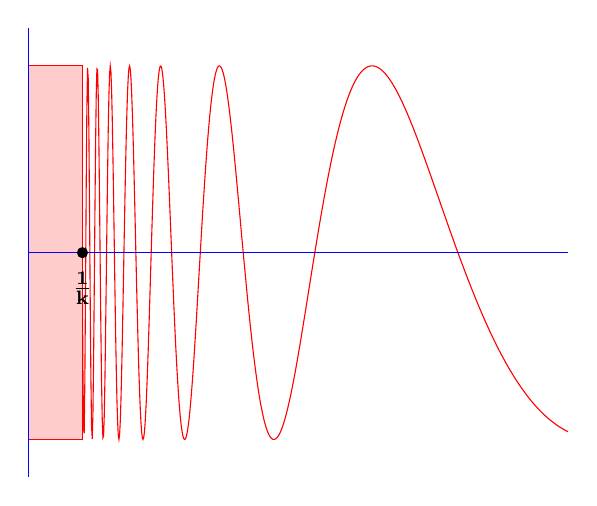
\begin{tikzpicture}
    \begin{axis}[axis lines=middle, xmin = 0 , ymin = -1.2 , ymax = 1.2 , xmax = 0.2, xtick=\empty, ytick=\empty, axis line style={color=blue, line width=0.6pt, -}, axis on top ]
      \addplot[domain=0.01:1, samples = 4000, color = red]{sin((deg(1/x)))};
      \addplot[draw=red, fill=red!20] coordinates {(0,-1) (0.02,-1) (0.02,1) (0,1)} \closedcycle ;
      \addplot[
  only marks,
  mark=*,
  mark size=1.8pt,
  color=black
] coordinates {(0.02,-0.00)};
\node[below] at (axis cs:0.02,-0.05) {$\mathbf{\frac1k}$};
    \end{axis}
  \end{tikzpicture}
  \caption{A picture of $\mathcal S_k$. The topologist's sine curve $\mathcal S$ is defined as the intersection of all such $\mathcal S_k$.}
\end{figure}

\section{The topologist's sine curve}
Because of \Cref{CauchyDfns} we can make the following definition:
\begin{definition}%[The topologist's sine curve]
  For $k:\mathbb N$, define $s_k:[\frac1k,1] \to [-1,1]$ by $s_k(x) = \sin(\frac1x)$ and $\mathcal S_k \subseteq [0,1] \times [-1,1]$ by 
  $$\mathcal S_k = ([0, \frac1k] \times [-1,1]) \cup graph(s_k)$$
  We define \textbf{the topologist's since curve} $\mathcal S = \bigcap_{k:\mathbb N} \mathcal S_k$. 
\begin{figure}[h!]
  \centering
  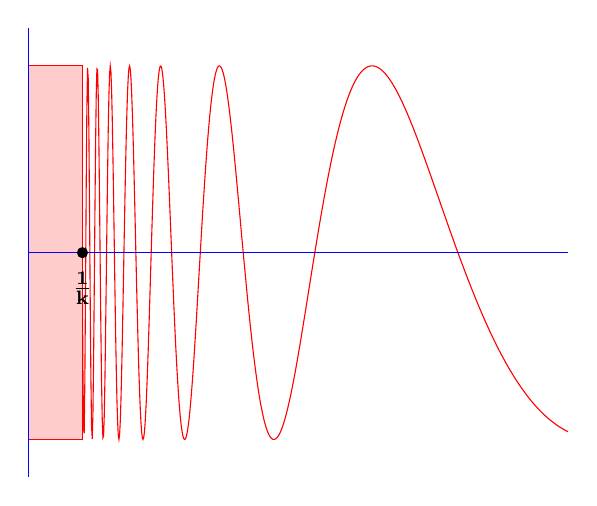
\begin{tikzpicture}
    \begin{axis}[axis lines=middle, xmin = 0 , ymin = -1.2 , ymax = 1.2 , xmax = 0.2, xtick=\empty, ytick=\empty, axis line style={color=blue, line width=0.6pt, -}, axis on top ]
      \addplot[domain=0.01:1, samples = 4000, color = red]{sin((deg(1/x)))};
      \addplot[draw=red, fill=red!20] coordinates {(0,-1) (0.02,-1) (0.02,1) (0,1)} \closedcycle ;
      \addplot[
  only marks,
  mark=*,
  mark size=1.8pt,
  color=black
] coordinates {(0.02,-0.00)};
\node[below] at (axis cs:0.02,-0.05) {$\mathbf{\frac1k}$};
    \end{axis}
  \end{tikzpicture}
  \caption{A picture of $\mathcal S_k$. The topologist's sine curve $\mathcal S$ is defined as the intersection of all such $\mathcal S_k$.}
\end{figure}

\end{definition}
  We shall denote $\iota_k : \mathcal S_k \to [0,1] \times [-1,1]$ 
  and $\iota:\mathcal S \to [0,1] \times [-1,1]$ for the inclusion maps, and $\pi_0:[0,1] \times[-1,1] \to [0,1],
\pi_1:[0,1] \times[-1,1] \to [-1,1]$ for the projection maps. 


\begin{lemma}
  The topologists's sine curve is a compact Hausdorff space.
\end{lemma}
\begin{proof}
  Note that both $[0,\frac1k] \times [-1,1]$ and $graph(s_k)$ are the image of compact Hausdorff spaces, hence closed by \Cref{CHausClosedImage}.
  By \Cref{ClosureClosedOpen} is follows that $\mathcal S$ is closed. We conclude by \Cref{CHausClosedImage}
\end{proof}

%\begin{remark}\label{NonZeroOnGraph}
%  Let $(x,y):[0,1]\times[-1,1]$. By \Cref{positiveNumbersCharacter}, if $(x,y)\in \mathcal S$ and $x \neq 0$, there is some $k:\N$ such that $x>\frac1k$ and hence $(x,y)\in \mathcal S_k$. 
%\end{remark}

%\begin{corollary}\label{NonZeroOnGraph}
%  By the above, if for some $x:[0,1] \times [-1,1]$ we have $x\in \mathcal S$ and $\pi_1(x)\neq 0$, there must be some $k\in\mathbb N$ with $x \in graph(t_k)$ and hence $\pi_2(x) =\sin(\frac1{\pi_1(x)})$. 
%\end{corollary}

\subsection{The curve is not path-connected}
\begin{remark}\label{topbottomSeq}
  For each $k:\N$, denote $t_k = \frac1{(2k+\frac12) \pi}$ and  $b_k = \frac1{(2k+\frac32) \pi}$. 
  Note that for all $k:\N$ we have $\sin(\frac1{b_k})=-1, \sin(\frac1{t_k})=1$ and
  $1>t_k>b_k>t_{k+1}>b_{k+1}>0$. 
\end{remark}
\begin{lemma}\label{cofinaltbseq}
  Given $r:[0,1]$ with $r>0$, there exists some $k:\N$ with $t_k,b_k<r$.  
\end{lemma}
\begin{proof}
  By \Cref{positiveNumbersCharacter}, there is some $k:\N$ with $\frac1k<r$. As $(2k+\frac32)\pi,(2k+\frac12)\pi>k$, this $k$ suffices.
\end{proof}
\begin{lemma}\label{NonZeroOnGraph}
  Let $(x,y):[0,1]\times[-1,1]$ be such that $(x,y)\in\mathcal S$ and $x>0$.
  Then $y = \sin(\frac1x)$
\end{lemma}
\begin{proof}
  By \Cref{positiveNumbersCharacter}, there is some $k:\N$ such that $x>\frac1k$ and hence $(x,y)\in \mathcal S_k$ and $y = \sin(\frac1x)$. 
\end{proof}

\begin{lemma}\label{SineWillHitTopBot}
  Let $\gamma:[0,1] \to \mathcal S$. 
  Assume that $\pi_1(\gamma(0)) = 0$ and $\pi_1(\gamma(r))>0$ for some $r:[0,1]$. 
  Then there exist some $u,v:[0,1]$ with $0<u<v<r$ such that $\pi_2(\gamma(u)) = 1$, and $\pi_2(\gamma(v)) = -1$. 
\end{lemma}
\begin{proof}
  By \Cref{cofinaltbseq}, there exists some $k:\N$ such that $0 < b_k<r$. 
  We can thus apply \Cref{IntermediateValue} to $\pi_1\circ \gamma : [0,1] \to [0,1]$ to find some $v:[0,1]$ with $\pi_1(\gamma(v)) = b_k$. Then by \Cref{NonZeroOnGraph} and \Cref{topbottomSeq} we find that $\pi_2(\gamma(v)) = -1$. 
  The case for $u$ is similar. 
\end{proof}

\begin{theorem}[The topologist's sine curve is not path-connected]
  There is no map $\gamma:[0,1] \to \mathcal S$ such that $\gamma(0) = (0,0)$ and $\gamma(1) = (1,sin(1))$. 
\end{theorem}
\begin{proof}
  By applying dependent choice to \Cref{SineWillHitTopBot}, 
  we can find sequences $u_i,v_i,~i:\N$ such that $\pi_2(\gamma(u_i)) = 1, \pi_2(\gamma(v_i)) = -1$ and 
  $u_{i+1}<v_{i+1}<u_i<v_i$ for all $i:\mathbb N$. 
  We now apply \Cref{UniformContinuity} for $\epsilon =2 $.
  There is some $\delta>0$ such that $d(u_i, v_j)\geq \delta$ for any $i,j:\mathbb N$ as  $d(\gamma(u_i), \gamma(v_j)) \geq 2$. 
  Therefore, the sequence $u_i$ is decreasing with steps of at least size $2\delta>0$. 
  But this means that for $N>\frac1{2\delta}$, we have $u_{N}<0$, while $u_N :[0,1]$, which is a contradiction. 
\end{proof}

\begin{remark}
  One could define an equivalence relation on any type $X$ such that 
  $x\sim y$ iff there is a path from $x$ to $y$. 
  The equivalence classes of this relation would normally be called the path-connected components. 
  We conjecture that the space of path-connected components of $\mathcal S$ is equivalent to the type of open propositions. 
\end{remark}

\subsection{The shape of the curve}
We will prove that $\mathcal S$ is $[0,1]$-contractible. 
\begin{remark}
  We denote for each $r:[0,1]$ the fiber 
  $\mathcal S_r:= (\pi_1\circ \iota)^{-r}$. 
  Note that 
  $\mathcal S_r = \mathcal S \cap (\pi_1^{-1}(r)) = 
  \mathcal S \cap (\{r\} \times [-1,1])$, and that $\mathcal S_r$ is closed for all $r:[0,1]$. 
\end{remark}


\begin{lemma}\label{fiberInhabited}
  $\pi_1\circ \iota : \mathcal S \to [0,1]$ is surjective.  
\end{lemma}
\begin{proof}
  We shall show that for each $r:[0,1]$ the fiber $\mathcal S_r$ is merely inhabited. 
%
  By \Cref{compactnessCHaus}, 
  it's sufficient to show that $\pi_1^{-1}(r) \cap \mathcal S_k$ 
  is merely inhabited for any $k:\mathbb N$. 
%
  Let $k:\mathbb N$. 
  As we're showing a proposition, we make for each $k:\N$ a case distinction based on \Cref{LLPO}:
%  Note that $r\leq \frac1k \vee r \geq \frac 1k$. 
  \begin{itemize}
    \item If $r\leq \frac1k$, we have that $(r,0) \in \mathcal S_k$. 
    \item If $r\geq \frac1k$, $\frac1r$ is well-defined and 
      $(r,\sin(\frac1r)) \in \mathcal S_k$. 
  \end{itemize}
  Hence in both cases we have that $\pi_1^{-1}(r) \cap \mathcal S_k$ is inhabited, as required. 
\end{proof}

\begin{lemma}
  For each $k:\mathbb N$ and $r:[0,1]$, $\mathcal S_k\cap \pi_1^{-1}(r)$ is convex. 
\end{lemma}
\begin{proof}
  Suppose that $(x,y), (x',y')$ both lie in $\mathcal S_k\cap \pi_1^{-1}(r)$. 
  Suppose furthermore that $\alpha,\beta:[0,1], \alpha+ \beta = 1$. 
  We will show that $\alpha\cdot (x,y) + \beta\cdot (x',y') $ also lies in 
  $\mathcal S_k \cap \pi_1^{-1}(r)$. 

  Recall that 
  $\mathcal S_k = [0,\frac1k] \times [-1,1]  \cup graph(s_k)$. 
  As we will show a proposition, we can make a case distinction 
  for both $(x,y), (x',y')$ on whether they come from $[0,\frac 1k] \times [-1,1]$ or 
  from $graph(s_k)$.
  \begin{itemize}
    \item 
      If either comes from $[0,\frac1k] \times [-1,1]$, we must have that 
      then $r \leq \frac1k$. 
      Then $\pi_1^{-1}(r) = \{r\} \times [-1,1]\subseteq \mathcal S_k$. 
      It follows that $\pi_1^{-1}(r) \cap \mathcal S_k = \{r\} \times [-1, 1]$, which is convex. 
    \item 
      If both come from $graph(t)$, 
      then $x = x' = r$ and $y = y' = \sin(\frac1r)$. 
      Hence $(x,y) = (x',y')$ and thus $\alpha(x,y) + \beta(x',y') = (x',y')$. 
  \end{itemize}
  In both cases we conclude that $\alpha (x,y) + \beta(x',y')$ lies in 
  $\mathcal S_k\cap \pi_1^{-1}(r)$. 
\end{proof}

\begin{corollary}\label{fiberConvex}
  For each $r:[0,1]$, the fiber 
  $\mathcal S_r$ is convex. 
\end{corollary}
\begin{proof}
  Any intersection of convex subspaces of $\mathbb R^n$ is itself convex
\end{proof}
\begin{theorem}
  $\mathcal S$ is $[0,1]$-contractible. 
\end{theorem}
\begin{proof}
%  We write $\mathcal S = \sum\limits_{r:[0,1]} \mathcal S_r$.
  By \Cref{fiberConvex} and \Cref{fiberInhabited}, each fiber $S_r$ is convex and inhabited, hence by \Cref{ConvexInhabitedToContractible} also $[0,1]$-contractible. 
%
  Thus both the maps $\pi_0 \circ i :\mathcal S \to [0,1]$ and $[0,1] \to 1$ have $[0,1]$-contractible fibers. 
  By \parencite[Lemma 1.33]{modalities}, so does their composite. 
  It follows that $\mathcal S$ is $[0,1]$-contractible. 
\end{proof}

\appendix

\printbibliography
\end{document}
